\chapter{Fundamentação Teórica}
\label{cap:fundamentacao-teorica}

    Neste capítulo serão abordados os temas que serviram como base para as nossas pesquisas, detalhando mais profundamente os paradigmas de inteligência ambiental. Em seguida, explicaremos superficialmente o conceito de inteligência artificial, sobretudo em \acrlong{sma}. E, por último, abordaremos os conceitos que a engenharia de sistemas utiliza para a construção de sistemas complexos nas mais diversas áreas de atuação.

\section{Inteligência Ambiental}
\label{sec:inteligência-Ambiental}

    O termo Inteligência Ambiental, \acrshort{ami}, foi introduzido  pelo comité Europeu \acrfull{istag}. Esse termo é usado para descrever ambientes onde artefatos computacionais se misturam ao plano de fundo, tornando o ambiente sensível e responsivo. O conceito de \acrshort{ami} teve como base a noção de  computação ubíqua, proposta por \citeonline{weiser1991computer}. Sua proposta era que, com o avançar da tecnologia, os computadores se tornariam cada vez menores, incorporando-se aos objetos do ambiente, até o momento em que se tornassem invisíveis para as pessoas. Assim, usuários estariam a todo momento interagindo com inúmeros dispositivos computacionais de forma discreta e simples. A Figura \ref{fig:computer_evolution} ilustra a evolução do volume de computadores com o passar do tempo.
    
    \begin{figure}[ht!]
        \centering
        \Caption{\label{fig:computer_evolution} Relação entre o número de pessoas e o número de computadores com o passar do tempo.} 
        \UECEfig{}{
            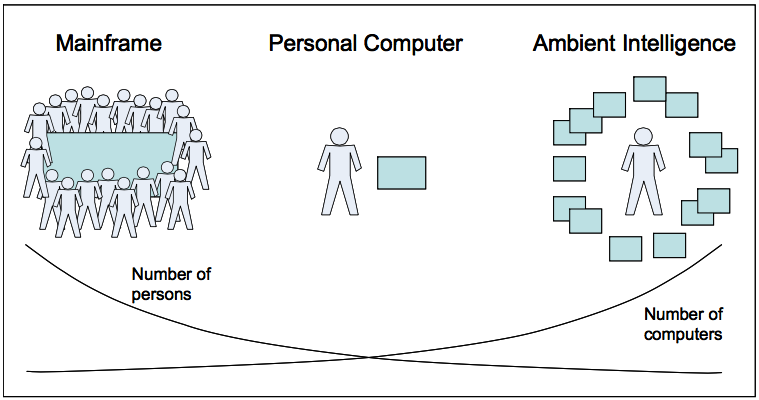
\includegraphics[width=8cm]{figuras/computer_evolution}
        }{
            \Fonte{\cite{bick2008ambient}}
        }   
    \end{figure}
    
    
    A computação ubíqua, ou computação pervasiva, apesar de ser fundamentalmente ligada à inteligência ambiental, possui uma diferença conceitual. A computação pervasiva enfatiza a presença de dispositivos físicos distribuídos pelo ambiente e a disponibilidade de recursos sem necessariamente tornar o ambiente inteligente \cite{augusto2007ambient}. A necessidade de uma inteligência comandando os recursos do ambiente é a pedra fundamental do conceito de ambientes inteligentes.
    
    %\subsection{Áreas da Inteligência Ambiental}
    
    Sistemas \acrshort{ami} se relacionam com diversas subáreas da ciência da computação, além da computação ubíqua e inteligência artificial. A grande quantidade de sensores exige uma robusta rede de comunicação. Além disso, a interação entre os dispositivos e as pessoas no ambiente deve ocorrer da forma mais transparente possível, através de interfaces que exijam o mínimo de esforço dos usuários. A inteligência artificial deve permear todas essas áreas, seja otimizando funções do sistema ou provendo mais facilidades ao usuário. A Figura \ref{fig:ami-relation} ilustra as diferentes áreas que fazem parte da inteligência ambiental.
    
    \begin{figure}[h!]
        \centering
        \Caption{\label{fig:ami-relation} Relação entre AmI e outras áreas.} 
        \UECEfig{}{
            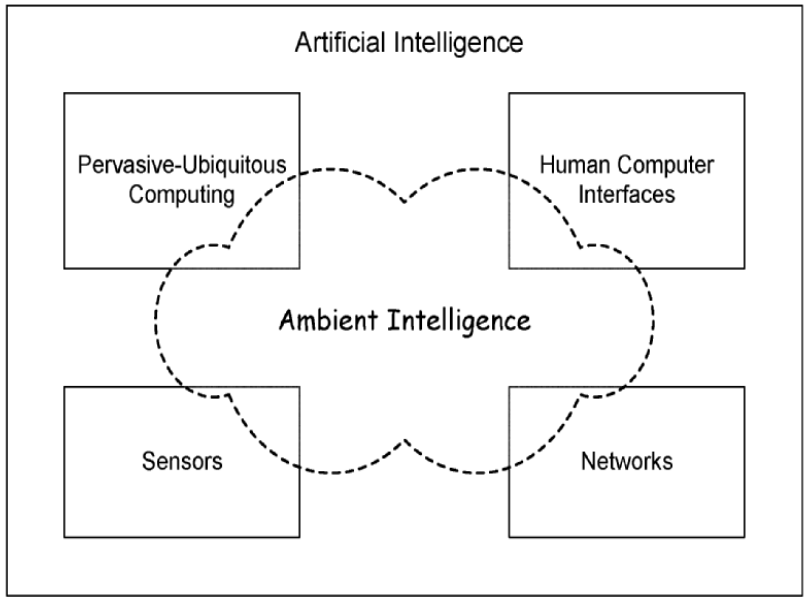
\includegraphics[width=6cm]{figuras/AMI-relations}
        }{
            \Fonte{\cite{augusto2007ambient}}
        }   
    \end{figure}
    
    A visão de um futuro cheio de objetos inteligentes e interativos oferece uma gama de oportunidades \cite{bohn2005social}. Ambientes inteligentes podem ser utilizados nos mais diversos contextos. Algumas áreas que podem e até já se beneficiam do uso de sensores e objetos inteligentes são listadas abaixo.
    
    \begin{itemize}
        \item \textbf{Aplicações relacionadas à saúde} -- Objetos inteligentes podem ser utilizados para fornecer serviços de monitoramento e análise dos pacientes de um hospital. Fornecendo aos médicos informações em tempo real do estado de cada um. 
        
        \item \textbf{Serviços de transporte} -- Carros inteligentes já estão em produção, e, apesar de ainda ser uma tecnologia muito nova, já mostra resultados animadores. Eles são equipados com sensores capazes de mapear o ambiente à sua volta e reconhecer outros carros próximos, evitando colisões e melhorando o fluxo de veículos. 
        
        \item \textbf{Serviços de educação} -- Instituições de ensino podem utilizar inteligência ambiental para monitorar seus alunos. Verificando sua frequência em sala de aula, acompanhando o progresso de suas atividades escolares, e, até mesmo, averiguando sua saúde.
        
        \item \textbf{Serviços de emergência} -- Serviços de emergência em geral podem ter um tempo de resposta melhor a um incidente. Por exemplo, casas equipadas com sensores de incêndio poderiam automaticamente enviar a sua localização aos bombeiros quando o fogo fosse detectado.
        
    \end{itemize}
    
    É interessante notar que os dispositivos utilizados em uma aplicação não necessariamente precisam estar no mesmo ambiente. Mais ainda, os objetos de uma aplicação podem ser utilizados não só por um, mas por vários sistemas. Por exemplo, digamos que um paciente esteja sendo monitorado em sua casa através de um conjunto de sensores; esses, por sua vez, enviam todas as informações captadas para o sistema do hospital através da internet. O sistema do hospital processa os dados  e, em caso de emergência, comunica à ambulância mais próxima a localização do paciente, enviando também as informações necessárias para socorrê-lo. Essa conexão entre vários ambientes inteligentes tornou-se possível graças à "\textit{Internet}das Coisas".
  
%\subsection{Internet das Coisas}
%\label{sec:internet-coisas}

    A \textit{Internet das Coisas}, \acrfull{iot}, é um fenômeno tecnológico derivado dos conceitos de comunicação ubíqua e inteligência ambiental \cite{dohr2010internet}. O termo \acrlong{iot} foi usado pela primeira vez no fim da década de noventa, no trabalho de \citeonline{ashton2009internet}, onde uma série de objetos eram capazes de se comunicar através de sensores \acrshort{rfid}, possibilitando uma cooperação entre eles. Com o passar do tempo, esse conceito foi ampliado, permitindo que a comunicação acontecesse por outros meios como a \textit{Internet}, fornecendo, assim, informações e serviços a usuários de diversos locais.
    
    De uma perspectiva mais sistemática, a \textit{Internet das Coisas} pode ser tratada como um sistema altamente dinâmico e radicalmente distribuído, composto por um grande número de objetos inteligentes, produzindo e consumindo informação \cite{miorandi2012internet}.  Esses objetos se comportam como interface entre o mundo real e o virtual. Eles são capazes tanto de sentir fenômenos físicos quanto de produzi-los, traduzindo-os em uma corrente de informações para o mundo virtual e agindo no ambiente físico através de atuadores quando certas condições são alcançadas. 

\section{Programas de Agentes Artificiais Racionais}
\label{sec:agentes}

    Um agente é uma entidade capaz de perceber seu ambiente de tarefa por meio de sensores e agir nele por meio de atuadores. O comportamento de um agente pode ser descrito em termos matemáticos por uma função do agente capaz de mapear qualquer sequência de percepções para uma ação especifica. A função do agente é implementada concretamente pelo programa do agente, que é executado em uma arquitetura adequada (dispositivo de computação com sensores e atuadores físicos). Idealmente, os agentes artificiais racionais, aqui decompostos em um programa de agente e em uma arquitetura, devem agir visando alcançar o melhor resultado esperado, avaliado de acordo com uma medida de desempenho \cite{norvig2004inteligencia}.
    
    \citeonline{norvig2004inteligencia} especificaram quatro tipos básicos de programas de agentes racionais que podem ser adaptadas para resolver problemas em diversos tipos de ambientes de tarefas difíceis. Esses programas incorporam os princípios subjacentes a quase todos os sistemas inteligentes, são classificados levando-se em consideração as informações empregadas no processo de tomada de decisão e as etapas componentes desse processo, ou seja, os agentes reativos simples e sua extensão baseados em modelos empregando regras condição-ação, e os agentes orientados por objetivo e sua extensão orientada por utilidade. Mais recentemente, esboçou-se uma estrutura para o agente com aprendizagem, isto é, a estrutura de um dos quatro tipos básicos com a capacidade de aprendizagem, conseguida pela integração à estrutura básica de três novas etapas à tomada de decisão. A Figura \ref{fig:agente-aprendizado} apresenta o esboço da estrutura do agente com aprendizagem.

    \begin{figure}[h!]
        \centering
        \Caption{\label{fig:agente-aprendizado} Modelo geral de agentes com aprendizado.} 
        \UECEfig{}{
            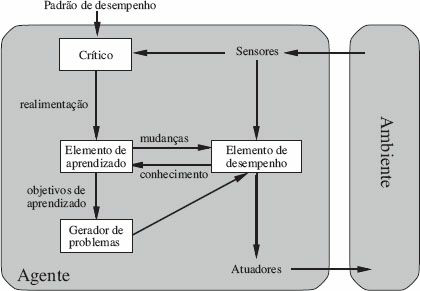
\includegraphics[width=6cm]{figuras/agente-aprendizado}
        }{
            \Fonte{\cite{norvig2004inteligencia}}
        }   
    \end{figure}

    \citeonline{wooldridge2009introduction} descreveu formalmente as arquiteturas abstratas do agente reativo e do agente com estado interno, considerando três subsistemas (módulos) de processamento de informação componentes. Em seguida, destacou quatro maneiras diferentes de se concretizar projetos de agentes racionais, ou seja, os agentes lógicos, \textit{subsumption}, \acrshort{bdi}, e com arquiteturas em camadas. A Figura \ref{fig:agente-estado} destaca os três módulos de processamento da informação na arquitetura abstrata do agente com estado interno.
    
    \clearpage
    \begin{figure}[h!]
        \centering
        \Caption{\label{fig:agente-estado} Modelo de um agente com estado interno.} 
        \UECEfig{}{
            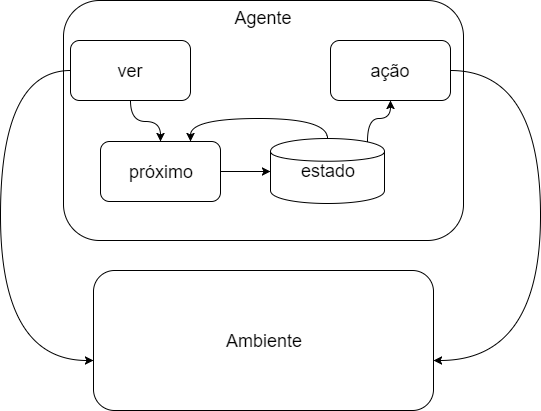
\includegraphics[width=6cm]{figuras/state-agent} %não sei se é a figura correta
        }{
            \Fonte{ Traduzido de \citeonline{wooldridge2009introduction}}
        }   
    \end{figure}
    

    O comportamento do agente com estado interno pode ser resumido da seguinte forma: o agente inicia a partir de algum estado interno \emph{i\textsubscript{0}}, então, observa o estado do seu ambiente \emph{e}, gerando a percepção \emph{ver(e)}. O estado interno do agente é assim atualizado com a função próximo($ver(e), i_0$). O agente então seleciona uma ação com base na função \emph{próximo} da seguinte forma \emph{ação(próximo(ver(e), i\textsubscript{0}))}. A ação é, portanto, executada, e, em seguida, inicia-se um novo ciclo, percebendo o ambiente através da função \emph{ver}, atualizando o estado interno com a função \emph{próximo}, e escolhendo uma ação com a função \emph{ação}. 

    \section{Organizações de Agentes Racionais}
    \label{sec:agent-org}
        
        \acrfull{sma} são conjuntos de agentes que interagem, cooperando para atingir um objetivo comum, ou competindo por recursos no mesmo ambiente. Nesse contexto, uma organização é um padrão de cooperação entre agentes predefinido pelo designer da aplicação, ou gerado pelos próprios agentes a fim de atingir um propósito comum \cite{boissier2004organization}. Em uma casa inteligente, por exemplo, o time de agentes que controla o ambiente deve cooperar para maximizar o conforto das pessoas que residem naquele espaço. 
        
        Mas, para que a organização funcione da melhor forma, é necessário que o projetista seja capaz de resolver dois problemas relacionados ao time de agentes. Primeiro: ele deve ser capaz de criar agentes heterogêneos que, além de agirem de forma individual, sejam capazes de cooperar. Segundo: ele deve criar uma organização racional para esses agentes. Para criar organizações de agentes é necessário descrever formalmente a organização \cite{francoempirical}.
        
    %\subsection{Organização Estrutural}
        \label{subsec:org-struct}
        Organizações representam a racionalização e ordenação de vários instrumentos a fins de se atingir um objetivo específico \cite{selznick1948foundations}. Para que esses objetivos sejam alcançados é necessário subdividi-los em diversos subobjetivos, que contribuem para o propósito geral da organização. Esses subobjetivos são definidos como papéis que são assumidos por agentes dentro de uma organização.
        
        Organizações em \acrshort{sma} são apresentadas normalmente como estruturas monodimensionais. No entanto, na maioria dos casos, são compostas por diversos aspectos estruturais: autoridade, comunicação, delegação, tomada de decisão, poder etc. No trabalho de \citeonline{grossi2005foundations}, as organizações são compostas por três dimensões, chamadas de: \emph{poder}, \emph{coordenação}, e \emph{controle}, onde o \emph{poder} está relacionado à delegação de atividades, a \emph{coordenação} se relaciona ao conhecimento ou compartilhamento de informações, e o \emph{controle} está ligado ao monitoramento de atividades. Formalmente, uma organização é representada pela tupla ilustrada a seguir. 
        
        \begin{equation}
            \centering
            \label{eq:os-structure}
            \langle  R, R_{power}, R_{coord}, R_{control}  \rangle
        \end{equation}
        
        Cada papel em uma organização é assumido por apenas um único agente. Essa imposição torna mais explícita e simples a relação de poder entre os papéis pertencentes à organização. 
        \emph{R} representa o conjunto de todos os papéis da organização e $R_{power}$,  $R_{coord}$, e $R_{control}$ são os relacionamentos entre papéis que caracterizam as estruturas de poder, coordenação, e controle. Tal que, $\forall{r, s}$ $\in$ \emph{R} temos que:
        \begin{equation}
            \label{eq:role-definition}
            \begin{split}
                 (r, s)  \in R_{poder} &\Rightarrow \exists \; R_{coord}(r, s);\\
                 (r, s)  \in R_{poder} &\Rightarrow \exists \;  t \in R \; | \; R_{control}(t, s)
            \end{split}
        \end{equation}
        
        A primeira parte da equação \ref{eq:role-definition} determina que, para toda relação de poder entre o papel \emph{r} e o papel \emph{s}, existe uma relação de coordenação de \emph{r} para \emph{s}. Isso implica que sempre deve haver um fluxo de informação relevante do agente que assume papel \emph{r} para o agente responsável pelo papel \emph{s}. Já na segunda parte da equação, para cada relacionamento de poder entre dois papéis, existe um papel \emph{t} responsável por controlar e monitorar suas ações. A Figura \ref{fig:os-graph} ilustra em um grafo os relacionamentos de uma estrutura organizacional, onde duas subestruturas, A e B, comunicam-se. 
        
        \clearpage
        \begin{figure}[h!]
            \centering
            \Caption{\label{fig:os-graph} Exemplo de uma estrutura organizacional.} 
            \UECEfig{}{
                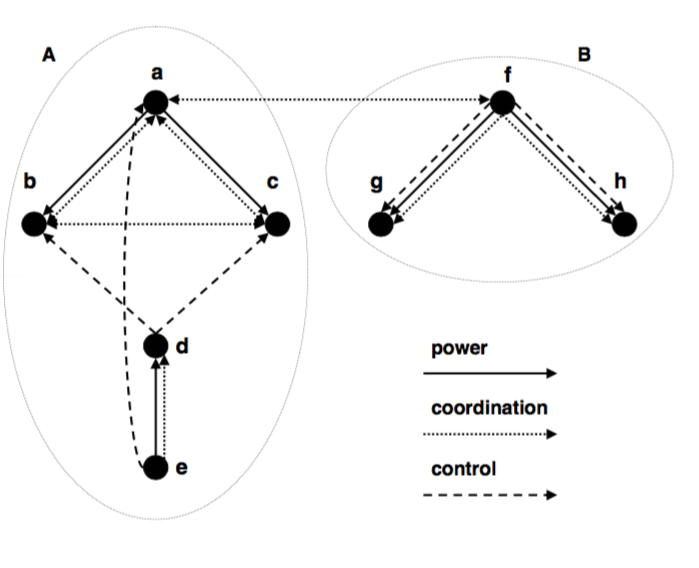
\includegraphics[width=6cm]{figuras/os-graph}
            }{
                \Fonte{ \cite{grossi2007structural}}
            }   
        \end{figure}
  
    % INSTITUIÇÕES ELETRONICAS FOI MOVIDO PARA TRABALHOS RELACIONADOS
            
  \section{Engenharia de Sistemas}
        
    O Conselho internacional de Sistemas e Engenharia (\acrshort{incose}) define engenharia de sistemas como uma abordagem interdisciplinar que permite a criação de sistemas. Ela se preocupa em: (1) definir as necessidades do usuário e seus requerimentos no início do ciclo de desenvolvimento; (2) documentar requerimentos; (3) proceder com a síntese de criação; e (4) validar o sistema considerando o problema como um todo. Para a engenharia de sistemas, a chave para a criação de sistemas bem-sucedidos, que satisfaçam os requisitos do cliente dentro de um espaço de tempo esperado, está na definição dos limites do sistema \cite{barry2009agent}.
    
    
    A engenharia de sistemas engloba todas as atividades envolvidas na aquisição, especificação, projeto, implementação, validação, implantação, operação e manutenção dos sistemas sociotécnicos \cite{sommerville2003engenharia}. Os engenheiros de sistemas se preocupam não apenas com o \textit{software}, mas também com o \textit{hardware} e com as interações entre o sistema, os usuários e o ambiente. Eles devem pensar sobre os serviços que o sistema oferece, as restrições sob as quais o sistema deve ser construído e operado e as maneiras pelas quais o sistema é usado para cumprir seu propósito ou finalidade.
    
    O modelo V, ilustrado na Figura \ref{fig:systems-vee}, representa um dos vários ciclos de vida da engenharia de sistemas. Na primeira parte, o modelo descreve detalhadamente o design dos subcomponentes do sistema, até o momento onde se atinge um entendimento mais completo do sistema e de como esses componentes trabalharão. Aí, os componentes são implementados e, em seguida, integrados e testados, até o ponto onde todo sistema esteja completo.
    
    \clearpage
    \begin{figure}[h!]
        \centering
        \Caption{\label{fig:systems-vee}Modelo V de desenvolvimento de sistemas.} 
        \UECEfig{}{
            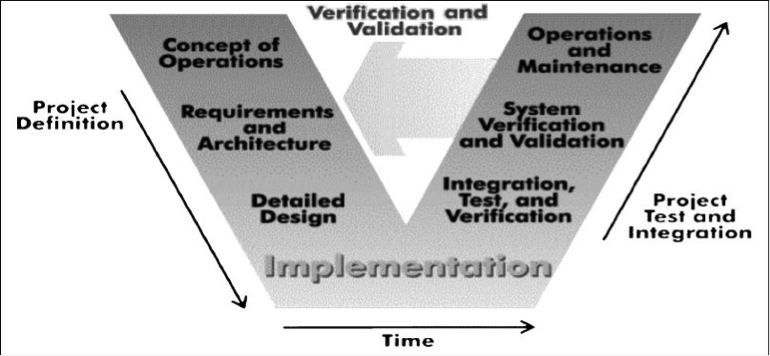
\includegraphics[width=8cm]{figuras/systems-vee}
        }{
            \Fonte{ \citeonline{barry2009agent}}
        }   
    \end{figure}
    
    O processo de desenvolvimento ilustrado na figura \ref{fig:systems-vee} é utilizado na Engenharia de Sistemas devido ao grande número de componentes sendo construídos simultaneamente. Para sistemas que incluem \textit{hardware} ou outros tipos de equipamentos físicos, alterações durante o desenvolvimento dos projetos acabam se tornando muito caras ou mesmo impossíveis. Isso torna necessário que os requisitos do sistema sejam assimilados pelo engenheiro antes de iniciar o desenvolvimento, ou construção, do \textit{hardware}. Porém, a medida que o sistema é instalado, podem ser identificadas limitações no projeto, sejam por problemas no \textit{hardware} ou por requisitos inalcançáveis. 

    Para evitar tal situação, é necessário criar algum projeto inicial para estruturar e organizar o processo de engenharia de requisitos. Nesse projeto, definiremos uma arquitetura de sistemas para, a partir dela, encontrar problemas com os requisitos existentes ou adicionar novos requisitos. Essa abordagem permite que o processo de definição de requisitos e de arquitetura seja tratado como algo contínuo na Engenharia de Sistemas. Consequentemente, podemos pensar nesses processos ligados em uma espiral, como mostra a Figura \ref{fig:espiral-requisitos}.
    
    \begin{figure}[h!]
        \centering
        \Caption{\label{fig:espiral-requisitos} Espiral de requisitos do projeto.} 
        \UECEfig{}{
            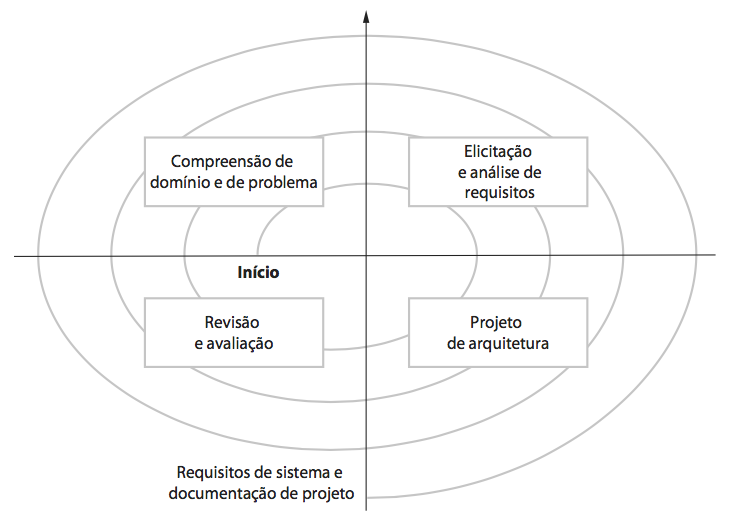
\includegraphics[width=8cm]{figuras/espiral-requisitos.png}
        }{
            \Fonte{ \citeonline{sommerville2003engenharia}}
        }   
    \end{figure}
     
    A espiral mostra como as decisões relacionadas a requisitos podem impactar no projeto e vice-versa. A partir de um ponto inicial, que representa a primeira versão do projeto, a espiral se afasta do centro, passando por todos os quadrantes do plano. Cada volta realizada representa uma nova adição ao projeto, ou um novo requisito.  
    
    De acordo com o Departamento de Defesa dos Estados Unidos \cite{dod2001systems}, a engenharia de sistemas é um processo de gestão interdisciplinar, que busca comprovar, integrar e evoluir um conjunto de soluções, balanceadas através de um ciclo de vida, que ofereçam saídas capazes de satisfazer o cliente. A gestão na engenharia de sistemas visa controlar e integrar os processos que estão sendo construídos. 
    
    %\subsection{Gestão da Engenharia de Sistemas}
        
    A gestão na engenharia de sistemas é alcançada através da integração de três outras atividades, a saber: fase de desenvolvimento; processo de engenharia de sistemas; e ciclo de vida e integração. Cada uma dessas atividades é essencial para atingir uma gestão adequada do desenvolvimento do sistema.
    
    A fase de desenvolvimento é responsável pela conexão entre o design do sistema e a criação, ou aquisição, de tecnologia. Esse processo de desenvolvimento pode ocorrer nos seguintes estágios: (a) em um nível conceitual, onde é produzido um conceito do sistema; (b) em nível de sistema, produzindo uma descrição sobre a performance dele em relação aos seus requisitos; e (c) em nível de subsistema/componente, gerando descrições dos subsistemas/componentes, indicando suas performances e, ainda, uma descrição detalhada das suas características.
    
    O processo de engenharia de sistemas é a etapa mais importante da engenharia de sistemas. O seu propósito é fornecer uma estrutura robusta e flexível, capaz de atender aos requisitos do sistema. Esse processo permite maior controle no desenvolvimento de soluções capazes de atender às necessidades do cliente. Esse procedimento é aplicado em cada nível de desenvolvimento do sistema para produzir uma descrição básica de configuração. Ele segue uma abordagem \textit{top-down}, resolvendo problemas de forma iterativa e recursiva, aplicada de forma sequencial em todos os estágios de desenvolvimento. Esse processo é utilizado para transformar requisitos em um conjunto de produtos do sistema e descrições do processo, adicionando mais detalhes ao desenvolvimento e mais valor, gerando mais informações para auxiliar na tomada de decisões.

    O ciclo de vida e integração se refere às ações associadas ao próprio ciclo de vida do sistema. Ele é necessário para garantir que a solução elaborada pelo sistema seja válida durante toda a sua execução. Essa etapa também inclui o planejamento associado ao desenvolvimento, assim como a integração das múltiplas funcionalidades relacionadas ao \textit{design} e ao processo de engenharia.

%\subsection{Processo de Engenharia de Sistemas}
%\label{subsec:proc-eng-sis}

    No processo de engenharia de sistemas, novas arquiteturas são criadas para descrever e compreender melhor o sistema. A palavra "arquitetura" é utilizada em diversos contextos dentro da engenharia de sistemas, geralmente para descrever como os subsistemas devem ser conectados. No entanto, segundo o \citeonline{dod2001systems}, existem três tipos de arquitetura que podem ser usadas para retratar as diversas características de um sistema, a saber: arquitetura funcional, arquitetura física, e arquitetura do sistema. 
    
    A arquitetura funcional identifica e estrutura os requisitos funcionais e não funcionais. A arquitetura física retrata o sistema final, quebrando-o em diversos subsistemas. A arquitetura de sistemas identifica todos os artefatos relevantes para construir o sistema, incluindo os processos necessários para apoia-lo.
    
    A Figura \ref{fig:sys-eng-process} mostra todas as etapas iniciais do processo de engenharia de sistemas. As atividades fundamentais são a análise de requisitos, análise e alocação funcional, e síntese de \textit{design}, todas coordenadas pelo sistema de análise e controle.
        
    \begin{figure}[h!]
        \centering
        \Caption{\label{fig:sys-eng-process} Processo de Engenharia de Sistemas.} 
        \UECEfig{}{
            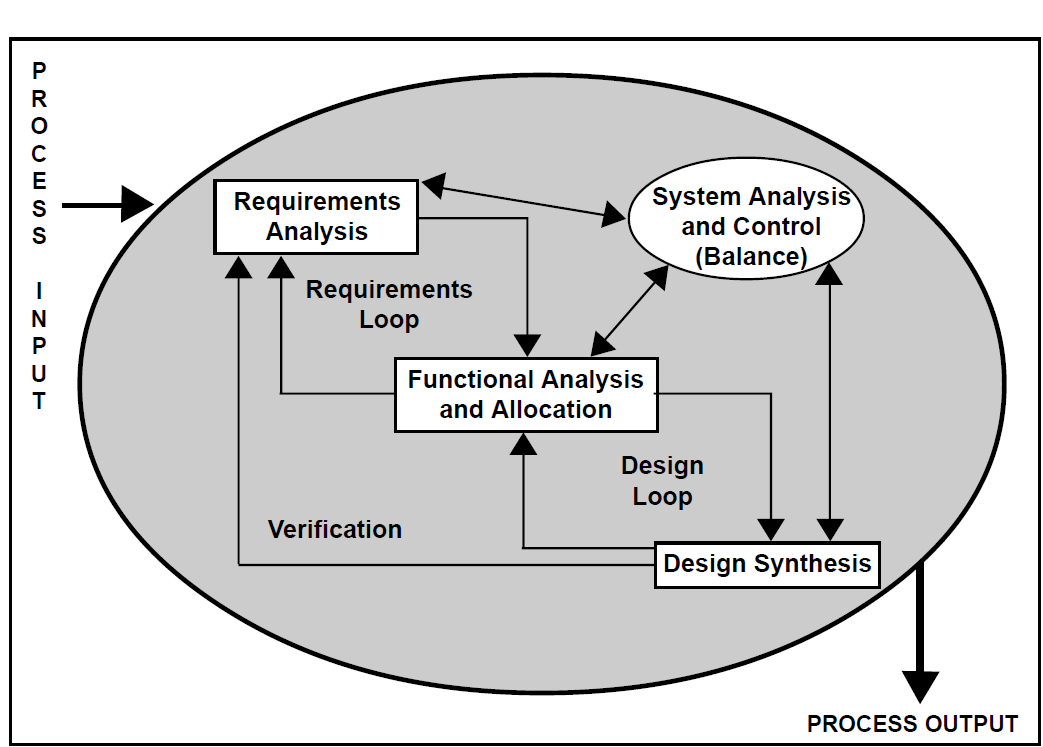
\includegraphics[width=7cm]{figuras/sys-eng-process}
        }{
            \Fonte{ \citeonline{dod2001systems}}
        }
    \end{figure}
    
    A primeira etapa do processo é analisar as entradas. A análise de requisitos é utilizada para desenvolver os requisitos funcionais e não funcionais. Ou seja, as exigências do cliente são traduzidas em um conjunto de requisitos que definem o que o sistema deve fazer e como deve ser seu desempenho. O engenheiro de sistemas deve assegurar que os requisitos sejam compreensíveis, inequívocos, abrangentes, completos e concisos.
    
    Com a análise de requisitos são identificadas funções de alto nível, que são decompostas em diversas funções de baixo nível durante a análise de função. Os requisitos de performance associados a funções de alto nível são alocados para funções de baixo nível. O resultado desse procedimento é uma descrição lógica do sistema em termos de performance. Isso também é conhecido como arquitetura funcional do sistema. A análise funcional e alocação possibilita um melhor entendimento daquilo que o sistema deve fazer, e de como fazer. Além de prover informações sobre as prioridades e conflitos associados às funções de baixo nível, fornecendo informações essenciais para a otimização de problemas físicos.
    
    O \textit{loop} de requisitos compara as funções analisadas e suas performances com seus respectivos requisitos, a fim de aproximar os resultados obtidos com aqueles definidos pelos requisitos. Esse é um processo interativo que revisa os requisitos à medida que sua análise é realizada. 
    
    A síntese de \textit{design} define o sistema em relação aos seus elementos de \textit{hardware} e \textit{software}. Esse processo também é chamado de "arquitetura física". Cada um dos componentes é responsável por, pelo menos, um requisito funcional, e qualquer parte pode ter diversas funções. A arquitetura física é a estrutura básica para definir os parâmetros de especificação do sistema.

    Com o fim da etapa de síntese, os resultados obtidos são comparados com os requerimentos da etapa de análise. Esse processo é chamado de "\textit{loop} de verificação". Cada requisito deve ser examinado. Como esse processo do sistema passa por diversas etapas de desenvolvimento, são necessários diversos métodos de verificação, sendo alguns deles: o exame, a demonstração, a análise (modelagem e simulação), e o teste.
    
    Os sistemas de análise e controle são compostos por técnicas de gestão de atividades necessárias para medir o progresso, avaliar e selecionar alternativas e tomar decisões. Essas atividades são aplicadas em todos os passos do processo de engenharia de sistemas.

\section{Descrevendo Sistemas em Níveis}
\label{sec:abord-def-nivel}

    Segundo \cite{wilensky1999thinking}, um sistema pode ser visto como uma unidade funcional devidamente concebida para realizar algum objetivo em algum ambiente. Especificando um pouco mais a ideia, esse tipo de sistema também pode ser visto como um conjunto de partes (componentes) interdependentes que trabalham juntas como uma só, visando realizar o objetivo original do sistema.% A Figura \ref{fig:nivel-1} exemplifica um sistema \acrshort{ami} composto por dois subsistemas. Um representando as pessoas e outro representando o sistema técnico, composto pelo hardware e software do sistema.%, com capacidade para satisfazer um objetivo próximo do objetivo original do sistema.
    
    %\begin{figure}[h!]
    %    \centering
    %    \Caption{\label{fig:nivel-1} Visão superficial de um sistema \acrshort{ami}} 
    %    \UECEfig{}{
    %        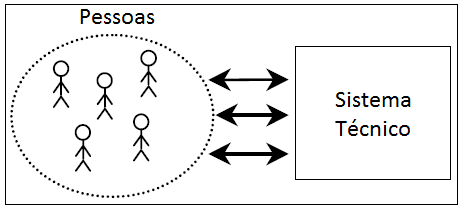
\includegraphics[width=6cm]{figuras/nivel-1}
    %    }{
    %        \Fonte{\cite{davidsson2000multi}}
    %    }   
    %\end{figure}
    
    A noção de níveis de descrição de sistemas historicamente vem sendo utilizada como meio para analisar e compreender uma ampla gama de sistemas naturais. Essa noção pode ser empregada para descrever e compreender melhor diversos tipos de sistemas, desde sistemas que estão em funcionamento atualmente quanto sistemas futuristas, que ainda não estão em funcionamento e são difíceis de projetar.
    
    A noção de nível que está sendo proposta é denominada "visão emergente" de níveis. Essa ideia é bastante diferente da noção de nível em sistemas vistos como hierarquias clássicas, onde o controle do sistema é identificado por meio de uma cadeia de comandos que flui de níveis mais altos para níveis mais baixos, como ilustra a Figura \ref{fig:hierarquia-classica}, em algumas organizações empresariais: o executivo-chefe está no nível superior, depois o presidente, em seguida o vice-presidente, e assim por diante.

    \begin{figure}[!ht]
        \centering
        \Caption{\label{fig:hierarquia-classica} Noção de níveis em uma hierarquia clássica.} 
        \UECEfig{}{
            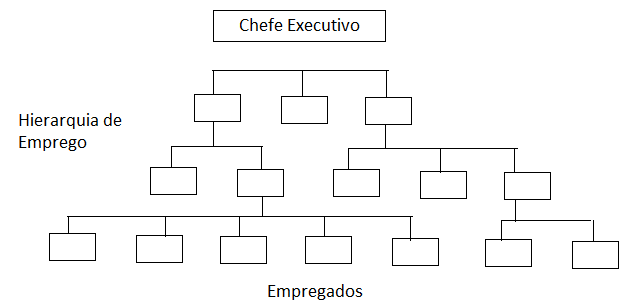
\includegraphics[width=8cm]{figuras/hierarquia-classica}
        }{
            \Fonte{Elaborado pelo autor}
        }   
    \end{figure}
    
    A noção de níveis emergentes, em vez de enxergar CEOs -- gerentes e trabalhadores de linha de montagem dentro de uma hierarquia --, enxerga e descreve uma organização empresarial em termos de divisões corporativas e dos funcionários dentro deles. Por exemplo, a Figura \ref{fig:box-system} ilustra de maneira genérica a descrição em níveis destacando um sistema composto de subsistemas inter-relacionados. Cada um desses subsistemas (A1-A3, B1-B2, C1-C3) pode ser descrito de maneira semelhante até que se atinja um determinado nível inferior de subsistemas elementares.
    
    \begin{figure}[h!]
        \centering
        \Caption{\label{fig:box-system} Diferentes níveis de um sistema simples.} 
        \UECEfig{}{
            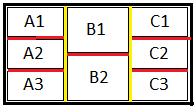
\includegraphics[width=6cm]{figuras/box-system}
        }{
            \Fonte{ Adaptado de \citeonline{simon1996sciences}}
        }   
    \end{figure}
     
    A noção de níveis emergentes é também diferente da noção de nível em sistemas vistos como contêineres, baseada na ideia de partes e todos. Por exemplo, um dia é parte de uma semana, logo, está em um nível mais baixo do que o nível de uma semana, que está em um nível mais baixo do que o nível de um mês, e assim por diante. A visão contêiner difere da visão hierárquica, em que os elementos de um nível inferior são partes dos elementos de um nível superior: um mês é parte de um ano, mas um vice-presidente não faz parte de um executivo-chefe. 
    
    A noção de níveis de descrição, conhecida como "visão emergente" de níveis, foca em fenômenos que surgem de interações de objetos em níveis inferiores. Por exemplo, em sistemas rodoviários urbanos, o engarrafamento que emerge das interações entre os carros nas ruas \cite{wilensky1999thinking}. Menos aparente que o engarrafamento, desempenho de uma divisão corporativa é resultado da complexa rede de relacionamentos e interações entre todos os seus funcionários.   
    Um dos pontos fundamentais quando se pensa em níveis emergentes está no entendimento da noção de comportamento emergente. %nesse caso seria o comportamento emergente inves do objeto???
    O comportamento emergente, ou objeto emergente, depende da forma com a qual o projetista se refere ao sistema. Enxergando o sistema como uma sociedade de (centenas, milhares, \ldots de) objetos separados que cooperam entre si, ou como um único objeto que, sob determinadas condições, pode se dividir em várias partes. Ou seja, o surgimento desse comportamento está relacionado à forma como o projetista enxerga o sistema: referindo-se a ele como como uma unidade, ou como o resultado da interação de diversos componentes, empregando o pronome "ele" ou "eles", ou o verbo "é" ou "são" \cite{wilensky1999thinking}.
    

    Objetos que são vistos como singulares em um nível podem ser melhor compreendidos como plural em outro nível. A capacidade de enxergar o mesmo objeto como singular ou plural, dependendo da situação, permitirá ao projetista de um sistema \acrshort{ami} construir uma compreensão científica mais profunda dos fenômenos intrínsecos ao sistema em desenvolvimento, o que pode ser uma informação valiosa para tomada de decisão na etapa de desenvolvimento
    
    Em sistemas naturais, por exemplo, muitas vezes o objeto emergente observado é descrito de maneira espacial. Isto é, uma aglomeração espacial de componentes (por exemplo, de células), que possui um padrão detectável na sua posição x-y. O padrão emergente não é detectável nas posições x-y, mas por outros parâmetros dos componentes do sistema. Como, por exemplo, a distribuição de velocidades/energias e os desempenhos associados aos componentes, como resultado de uma rede complexa de relacionamentos e interações entre todos os componentes. A Figura \ref{fig:gas-exemplo} ilustra esta ideia para o caso do comportamento de um gás em um recipiente selado. 
    
    \begin{figure}[h!]
        \centering
        \Caption{\label{fig:gas-exemplo} Padrão de comportamento das partículas de um gás.} 
        \UECEfig{}{
            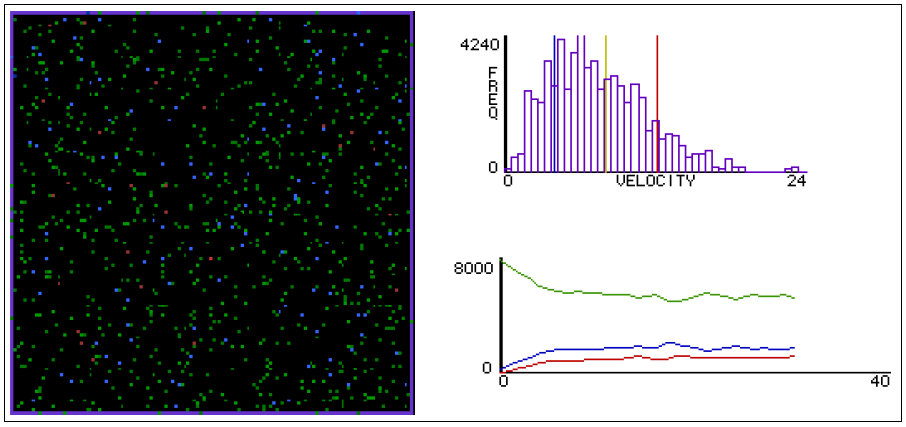
\includegraphics[width=8cm]{figuras/gas-exemplo}
        }{
            \Fonte{\citeonline{wilensky1999thinking}}
        }   
    \end{figure}
    
    
    No exemplo acima, centenas de partículas se encontram em um recipiente fechado. Elas se comportam como bolas de bilhar, colidindo de forma elástica quando se encontram ou quando se chocam com as paredes do recipiente. Todas as moléculas de gás do experimento iniciam em uma mesma velocidade (coloridas em verde). À medida que colidem podem acelerar (se colorindo de vermelho) ou desacelerar (coloridas em azul). Esse experimento foi realizado com intuito de ilustrar a distribuição de Maxwell-Boltzmann. Após um número de interações, a quantidade de partículas azuis (lentas) aumenta e a velocidade das partículas vermelhas cresce, de forma que a energia do gás como um todo permanece constante. Essa reação continua até o momento em que as velocidades se estabilizam, formando as distribuições ilustradas na Figura \ref{fig:gas-exemplo}.

    Assim como no caso dos sistemas naturais, parâmetros associados a componentes que são observados ao longo do tempo são um padrão mais difícil de detectar, resultando em um objeto emergente que é menos perceptível e menos óbvio. No entanto, uma distribuição de velocidades em um sistema \acrshort{ami} e uma aglomeração espacial, como as partículas de um gás, de componentes em um sistema natural, estão na mesma categoria, ou seja, fundamentalmente ambos podem ser vistos como objetos emergentes.
  
\begin{comment}


\section{Moise}
\label{sec:moise}

    A linguagem de modelagem organizacional Moise \cite{hubner2002model, hubner2007developing} descreve formalmente uma organização de agentes. Essa organização pode ser descrita através da especificação organizacional, \acrfull{os}, que pode ser dividida em três dimensões, \acrfull{ss}, \acrfull{fs}, \acrfull{ds}. A especificação estrutural (\acrshort{ss}) determina os papéis e seus relacionamentos, além dos grupos que compõem a organização. A especificação funcional (\acrshort{fs}) define os objetivos globais e o modo como eles serão alcançados. E por fim, a especificação deôntica (\acrshort{ds}) relaciona essas duas dimensões, identificando qual conjunto de objetivos e funções da camada funcional será atribuído a cada papel da camada estrutural. 

    %VERIFICAR NOMES DOS RELACIONAMENTOS STRUCTURAL SPECIFICATION
    Mais precisamente, a especificação estrutural é construída em três níveis, individual, social, e coletivo. No nível individual a \acrshort{ss} determina qual papel cada agente deverá assumir e quando. O nível social determina o relacionamento entre os papéis, sendo que os três tipos de relacionamento são: $authority$, $comunication$, e $acquaintance$. Onde um relacionamento $authority$ entre papéis implica na existência de uma ligação de $comunication$, que por sua vez implica numa relação de $acquaintance$ entre os papéis. E no nível coletivo a especificação estrutural define em quais grupos os papéis serão agregados.
    
    Essas descrições do \acrshort{ss} indicam um subconjunto de papéis que devem ser representados no grupo e sua cardinalidade miníma e máxima, representando a quantidade de agentes que podem assumir o mesmo papel simultaneamente. Além de definir subgrupos e relacionamentos com outros grupos. A Figura \ref{fig:moise-franco}(a) ilustra uma \acrshort{ss} do \emph{Moise} onde um grupo de agentes \emph{Gr} pode assumir dois papéis distintos, \emph{C} e \emph{S}, e um outro grupo de agentes pode assumir o papel \emph{L}. 
    
    \begin{figure}[h!]
        \centering
        \Caption{\label{fig:moise-franco}Estrutura organizacional de um time de agentes.} 
        \UECEfig{}{
            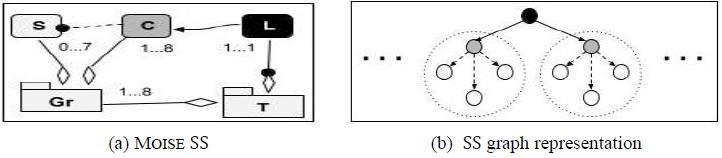
\includegraphics[width=10cm]{figuras/moise-franco}
        }{
            \Fonte{ \cite{francoempirical}}
        }   
    \end{figure}
    
    A partir da especificação estrutural do Moise podemos estabelecer uma relação entre os papéis de agentes na forma de um grafo, onde os papéis de agente são os vértices e os relacionamentos entre os papéis ($authority$, $comunication$, e $acquaintance$) são as arestas. o grafo da Figura \ref{fig:moise-franco}(b) representa a estrutura organizacional do time gerada a partir da \acrshort{ss} da Figura \ref{fig:moise-franco}(a).
    
\section{Instituições Eletrônicas}
\label{sec:fund-org-ei}
    %%%organizar e escrever o que for necessario!!!!!
    O comportamento de um sistema é definido pela forma como seus elementos relacionam, seja para atingir um determinado objetivo ou competir por um conjunto de recursos. Para definir formalmente esse comportamento, precisamos de um protocolo capaz de descrever todos os tipos de mensagens que os componentes de um \acrshort{sma} enviem entre-si. Para descrever  esse processo utilizamos uma versão mais sofisticada de uma máquina de estado não determinística, também conhecida como \acrfull{ei} \cite{rodriguez1999towards}.
    
    Essa semelhança com máquinas de estado finito confere a \acrshort{ei} diversas vantagens para a formalização de protocolos de interação. Existem diversas técnicas que automatizam o processo de verificação de propriedades de um determinado estado. Por exemplo, não devem existir estados que um agente jamais deve alcançar, ou estados onde uma vez alcançados não exista mais saída. Essas propriedades podem ser observadas com algoritmos básicos de teoria dos grafos.
    
    Neste trabalho utilizaremos uma versão simplificada da \acrshort{ei} utilizada no trabalho de \citeonline{vasconcelos2002approach}. Nessa versão simplificada a \acrshort{ei} é formada por um conjunto de \emph{cenas} conectadas através de \emph{transições}. Assumindo que exista uma linguagem de comunicação \emph{CL} entre os agentes e instituição eletrônica, uma \emph{cena} pode ser definida da seguinte forma:
    
    Para ilustrar melhor essa definição, a Figura \ref{fig:agora-exemplo} ilustra um exemplo de uma cena para \emph{agora room} \cite{miller1988markets}. Neste exemplo temos um agente comprador interagindo com uma série de agentes vendedores. Essa cena foi simplificada removendo negociações e leilões. O comprador anuncia os produtos que tem interesse, verifica as ofertas dos vendedores e escolhe a mais barata. 
    
    \begin{figure}[h!]
        \centering
        \Caption{\label{fig:agora-exemplo} Exemplo de cena} 
        \UECEfig{}{
        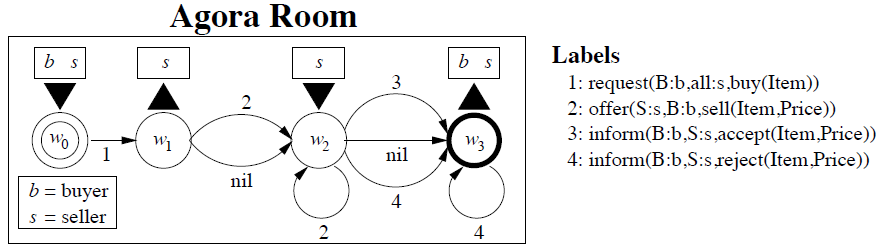
\includegraphics[width=12cm]{figuras/agora-exemplo}
        }{
        \Fonte{\cite{vasconcelos2002approach}}
        }   
    \end{figure}
    
    Na cena temos dois papéis, \emph{b} e \emph{s} representando respectivamente comprador e vendedor. O estado inicial $w_0$ é representado pelo par de círculos concêntricos, e estado final $w_3$ é simbolizado pela circulo mais denso. Os estados de acesso são marcados pelas caixas contendo os papéis e setas apontados para baixo, e os estados de saída são marcados pelas setas apontando para os papéis. Agora que definimos uma cena podemos definir uma \acrlong{ei}.
    
    \begin{theorem}
        Uma \acrshort{ei} é uma tupla $\varepsilon = \langle SC, T, S_0, S_\Omega, E, \lambda_E \rangle$ onde:
        \begin{itemize}
            \item SC = \{$s_1, \ldots, s_n$\} é um conjunto de finito não vazio de cenas;
            \item T  = \{$t_1, \ldots, t_m$\} é um conjunto finito e não vazio de transições;
            \item $s_0 \in SC$ é a cena raiz;
            \item $S_\Omega \in SC$ é a cena de saída;
            \item $E = E^I \cup E^O$ é um conjunto de arcos tal que $E^I \subseteq WE^S \times T$ é um conjunto de arestas dos estados de saída $WE^S$ da cena S, e $E^O \subseteq T \times WA^S$ é o conjunto de arestas de entrada dos estados $WA^S$ da cena S;
            
            \item $\lambda_E : E \mapsto p(x_1, \ldots, x_k)$ mapeia cada transição para um predicado correspondendo a suas restrições.
        \end{itemize}
    \end{theorem}
    
    As transições são conexões entre cenas pelas quais os agentes se movem, possivelmente trocando papéis e sincronizando seus movimentos com outros agentes. A Figura \ref{fig:ei-example} ilustra a definição acima através de um exemplo mais complexo do \emph{agora market} \cite{miller1988markets}. Essa \acrshort{ei} exige que os agentes passem por uma etapa de admissão antes de entrarem para o mercado, depois que a \emph{agora room} é finalizada compradores e vendedores quitam suas dívidas. 
    
    \begin{figure}[h!]
        \centering
        \Caption{\label{fig:ei-example} Exemplo de instituição eletrônica} 
        \UECEfig{}{
        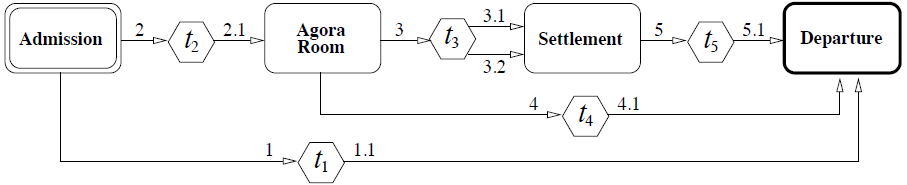
\includegraphics[width=12cm]{figuras/ei-example}
        }{
        \Fonte{\cite{vasconcelos2002approach}}
        }   
    \end{figure}
    
    Cada cena da instituição eletrônica é representada pelos retângulos de bordas arredondadas, onde o retângulo duplo representa a cena inicial, e o retângulo com bordas mais grossas caracteriza a cena final. Cada transição é simbolizada por hexágonos, e as linhas que ligam transições à cenas são os estados de saída ou acesso. 
    

\end{comment}